
\documentclass[tikz]{standalone}

\tikzstyle{treenode} = [draw,circle,minimum width=1.25em,font=\scriptsize,text centered,
inner sep=1.2pt,outer sep=0pt]

\begin{document}

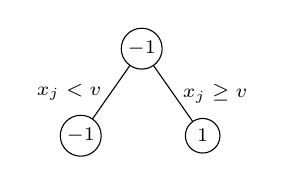
\begin{tikzpicture}
	\tikzset{help lines/.append style=pink}
%	\draw [help lines] (-2,-2) grid (2,1);
	
	\node[treenode] (root) at (0,0) {$-1$};
	\node[treenode] (root-l) at (-125:1.35) {$-1$};
	\node[treenode] (root-r) at (-55:1.35) {$1$};
	
	\draw[-] (root) -- node[font=\scriptsize,left] {$x_j<v$} (root-l);
	\draw[-] (root) -- node[font=\scriptsize,right] {$x_j\geq v$} (root-r);
\end{tikzpicture}

\end{document}
